\chapter{Planificación y gestión del proyecto}
\label{chap:planificacion}

\section{Metodología de desarrollo}
\label{sec:planificacion-metodologia}

El desarrollo de este trabajo ha seguido un enfoque incremental e iterativo combinado con una metodología experimental, sin adoptar formalmente Scrum, Kanban u otra metodología de trabajo ágil. La organización del trabajo se ha basado en el despliegue y la configuración de los servicios que componen la plataforma, su prueba en el clúster HPMoon y la revisión de las decisiones a partir de los resultados obtenidos.

El proceso no fue estrictamente lineal. Para automatizar un conjunto de pruebas fue necesario disponer previamente de un muestreador y de cargas ejecutables; a su vez, las primeras ejecuciones pusieron de manifiesto limitaciones que no podrían detectarse mediante pruebas locales. La integración con SLURM, los servicios remotos y el uso del medidor Vampire obligaron a alternar el análisis del entorno, la implementación, y el diagnóstico, ya que algunas incidencias solo podían detectarse al ejecutar el sistema en HPMoon. Tras cada corrección fue necesario repetir las ejecuciones para comprobar que el problema se había resuelto y que el flujo completo seguía funcionando correctamente.

Este enfoque resulta adecuado para un proyecto que combina software e infraestructura experimental. El correcto funcionamiento de los servicios que componen la plataforma puede verificarse de forma aislada mediante pruebas automáticas e individuales, pero la validez del flujo completo depende también de condiciones externas: disponibilidad del clúster, permisos, asignación del nodo, cobertura temporal de las muestras y correspondencia física del instrumento. Por ello, los resultados de cada iteración sirvieron para mejorar el sistema y revisar el diseño experimental.

\section{Organización del trabajo}
\label{sec:planificacion-fases}

El trabajo se ha organizado en las fases resumidas en la tabla~\ref{tab:fases-proyecto}. En cada fase se indican sus objetivos y resultados sin reproducir el diseño técnico del capítulo~\ref{chap:implementacion}.

\begin{table}[H]
    \centering
    \small
    \caption{Fases principales del desarrollo.}
    \label{tab:fases-proyecto}
    \begin{tabular}{p{0.20\textwidth}p{0.38\textwidth}p{0.31\textwidth}}
        \hline
        Fase & Actividades principales & Resultados de la fase \\
        \hline
        Estudio y acceso al entorno & Revisión de HPC, RAPL y SLURM; familiarización con HPMoon; primeras reservas y lecturas. & Configuraciones iniciales, trabajos de prueba y muestreador RAPL. \\
        Prototipo experimental & Implementación de cargas, ejecuciones individuales, persistencia inicial y publicación de métricas. & Orquestador individual, plantillas SLURM y primeros resultados. \\
        Automatización y perfiles & Generación de matrices, repeticiones, perfiles de CPU y campañas preliminares de Idle, memoria y cálculo. & Generador de matrices, configuraciones de campaña y resultados trazables. \\
        Observabilidad y análisis & Integración con Pushgateway, Prometheus y Grafana; consultas, paneles de control y análisis de correlación. & Módulo de monitorización, paneles de control y scripts de análisis. \\
        Medida externa & Integración de Vampire, sincronización con SLURM, descarga, validación de cobertura y publicación conjunta. & Módulo de integración, diagnósticos, pruebas y métricas externas. \\
        Validación final & Verificación de la configuración física, ejecución de la campaña definitiva y recálculo desde las muestras. & Dataset del 23/07, 61 ejecuciones válidas, tablas y figuras reproducibles. \\
        Documentación y revisión & Consolidación de decisiones, procedimientos remotos, limitaciones, memoria y anexos. & Documentación técnica, scripts de diagnóstico y memoria LaTeX. \\
        \hline
    \end{tabular}
\end{table}

Las fases presentan dependencias claras. La automatización se apoya en el prototipo de ejecución individual; la monitorización utiliza las métricas resumidas que ya han sido calculadas y almacenadas durante las ejecuciones; y la validación externa necesita marcas temporales compartidas entre el orquestador y el trabajo. El análisis definitivo se realizó después de fijar la campaña y sus controles de calidad, evitando adaptar retrospectivamente los datos brutos.

\section{Planificación temporal}
\label{sec:planificacion-temporal}

\subsection{Planificación inicial}
\label{subsec:planificacion-inicial}

Se hizo una planificación general inicial que fue concretándose conforme se fueron identificando las restricciones de HPMoon y de los medidores utilizados. Al no haberse creado inicialmente un calendario detallado con la dedicación y los criterios de aceptación, las fechas se presentan con precisión mensual.

El desarrollo se organizó de forma progresiva, de manera que cada fase se apoyaba en la anterior: primero se estudió el entorno, después se obtuvo una medida mediante RAPL, se ejecutaron cargas controladas, se automatizaron las repeticiones, se almacenaron los resultados y, finalmente, se habilitó su consulta. La integración externa y el análisis estadístico se incorporaron sobre ese flujo una vez estabilizadas sus interfaces principales.

La figura~\ref{fig:gantt-proyecto} representa la evolución temporal del proyecto entre marzo y julio y muestra el solapamiento entre sus principales fases. Dado que la planificación inicial se definió de forma general y se fue ajustando durante el desarrollo, el cronograma se presenta con una escala mensual y refleja de manera aproximada el trabajo realizado.

\begin{figure}[htbp]
    \centering
    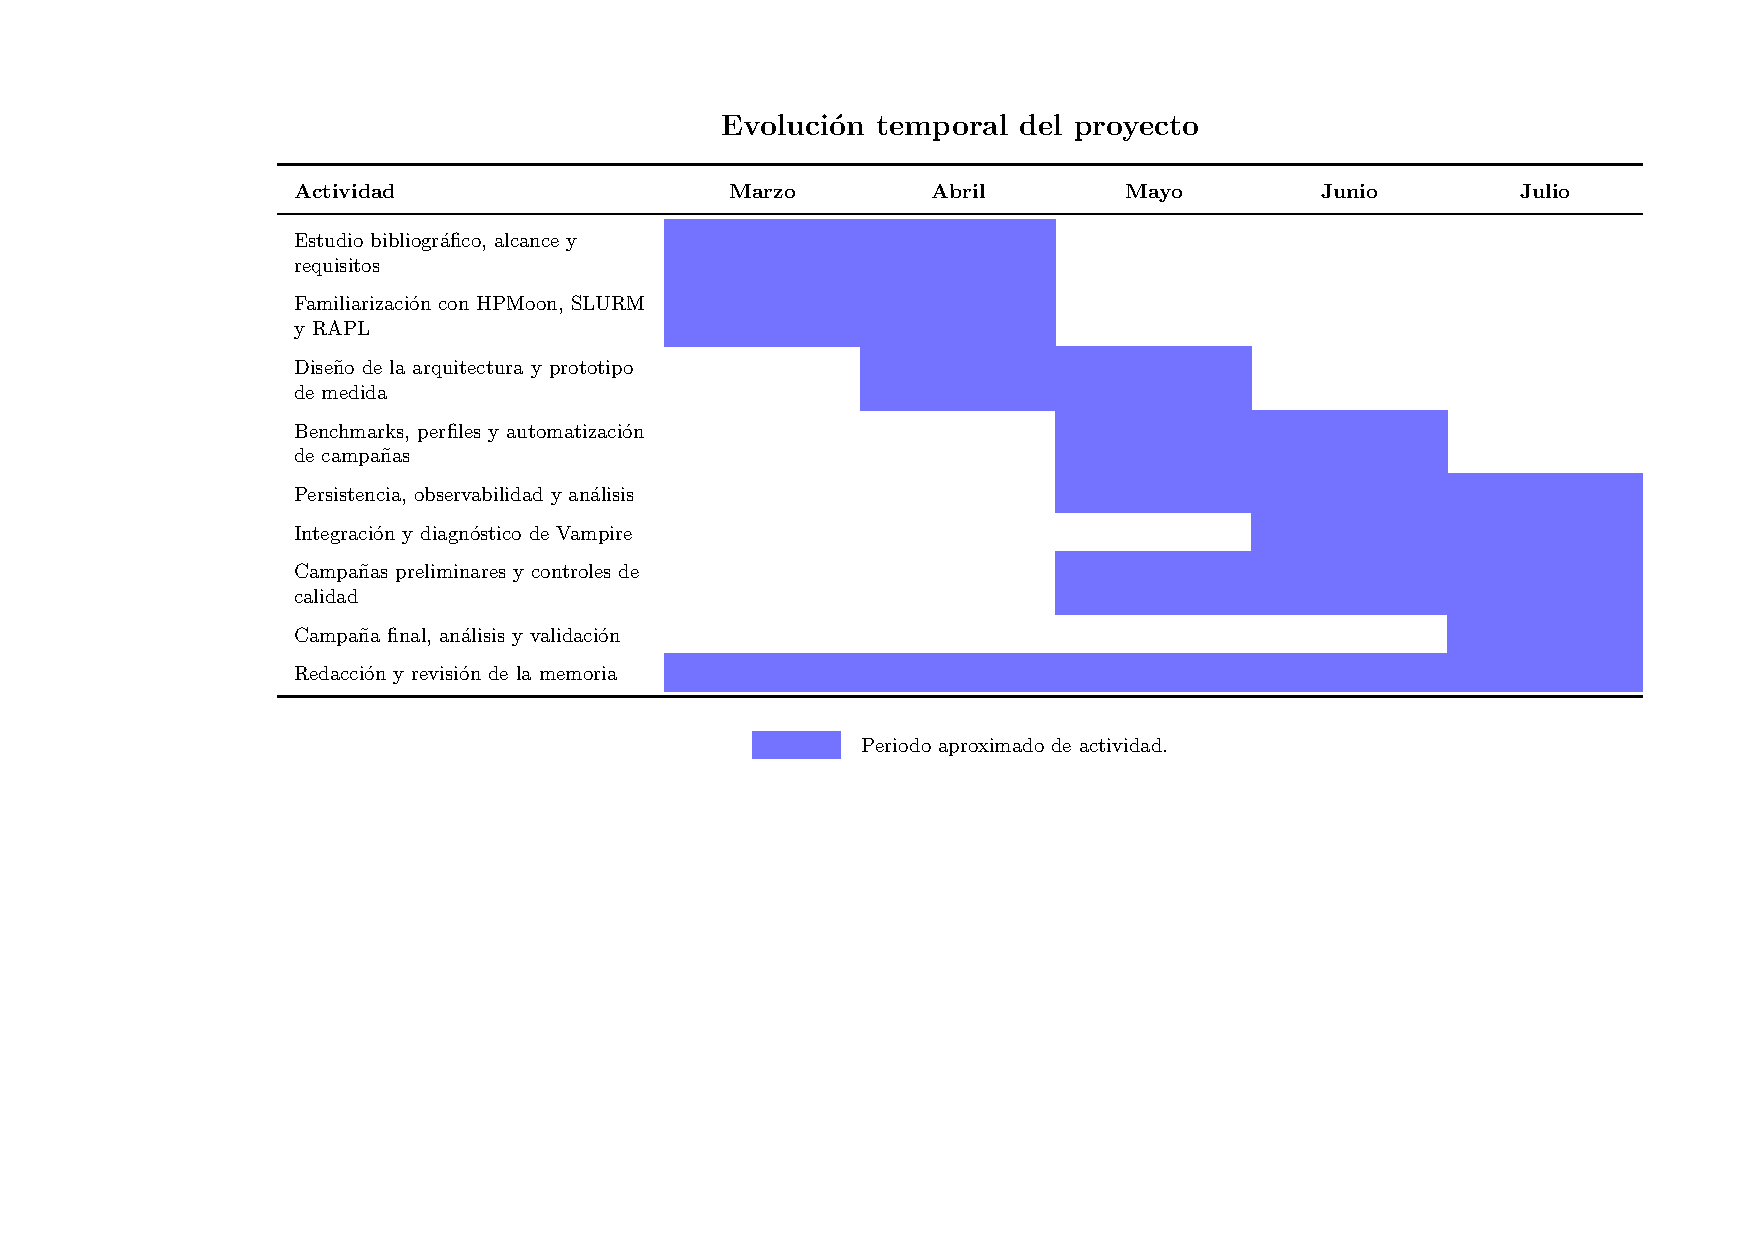
\includegraphics[width=\textwidth]{imagenes/capitulo7/gantt_proyecto.pdf}
    \caption{Evolución temporal aproximada del proyecto entre marzo y julio de 2026.}
    \label{fig:gantt-proyecto}
\end{figure}

El proyecto comenzó con el estudio del entorno HPMoon, el acceso al clúster y la revisión de las herramientas disponibles para la ejecución de trabajos y la medición energética. A partir de esta base se desarrolló un primer prototipo capaz de ejecutar una carga de forma controlada y obtener medidas mediante Intel RAPL. Posteriormente se incorporó la automatización de perfiles, repeticiones y almacenamiento de resultados, lo que permitió pasar de ejecuciones individuales a campañas experimentales completas.

Durante junio se realizaron campañas preliminares orientadas a comprobar el funcionamiento del sistema y a detectar posibles problemas en la adquisición y organización de los datos. Estas ejecuciones se solaparon con el desarrollo del análisis de resultados y con la incorporación de mecanismos de monitorización mediante Prometheus y Grafana. En julio se concentró la integración de la medida externa mediante Vampire, la corrección de incidencias relacionadas con la sincronización y la asociación entre nodo y dispositivo, y la ejecución de la campaña definitiva utilizada en el análisis final.

La documentación se desarrolló de forma paralela al resto del proyecto, recogiendo tanto las decisiones de diseño como la evolución de la implementación, los problemas encontrados y los resultados obtenidos.

\subsection{Principales ajustes durante el desarrollo}
\label{subsec:planificacion-real}

En la tabla~\ref{tab:periodos-desarrollo} se muestra el desarrollo del trabajo 

por meses e hitos funcionales. Los intervalos son aproximados y describen la secuencia y el solapamiento del trabajo, pero no constituyen un registro horario detallado.

\begin{table}[H]
    \centering
    \small
    \caption{Periodos aproximados e hitos principales del desarrollo.}
    \label{tab:periodos-desarrollo}
    \begin{tabular}{p{0.19\textwidth}p{0.30\textwidth}p{0.40\textwidth}}
        \hline
        Periodo aproximado & Trabajo predominante & Resultado principal \\
        \hline
        Marzo--abril & Estudio del problema, delimitación del alcance, familiarización con HPMoon, SLURM y RAPL. & Requisitos y planteamiento inicial de la infraestructura experimental. \\
        Abril--mayo & Diseño de la arquitectura, prototipo de muestreo, cargas controladas y ejecución individual. & Muestreador RAPL, programas de pruebas y primer flujo completo de ejecución. \\
        Mayo--junio & Automatización de matrices, perfiles, persistencia, campañas preliminares y observabilidad. & Configuraciones de campaña, resultados trazables, publicación y paneles de control. \\
        Junio--julio & Integración de Vampire, sincronización, controles de cobertura y diagnóstico de inconsistencias. & Integración externa reforzada, reintentos y herramientas de diagnóstico. \\
        Julio & Verificación de la configuración física, campaña definitiva y análisis. & Paquete validado del 23/07, tablas, figuras y resultados reproducibles. \\
        Marzo--julio & Redacción progresiva y revisión de la memoria. & Memoria LaTeX, anexos y documentación técnica consolidada. \\
        \hline
    \end{tabular}
\end{table}

Las desviaciones más relevantes fueron las siguientes:

\begin{description}
    \item[Acceso al Pushgateway.] La configuración inicial necesitó varios ajustes de dominio, ruta y uso de HTTPS. La consecuencia fue retrasar la estabilización de la observabilidad, sin afectar a los CSV locales. Se mantuvieron los datos almacenados localmente como fuente experimental y la publicación remota como una etapa separada.

    \item[Control de afinidad.] Se diseñaron perfiles utilizando \texttt{numactl}, una herramienta de Linux que permite controlar la asignación de procesos y memoria en sistemas NUMA, y se solicitó la opción \texttt{cpu-bind} de SLURM, utilizada para asociar los procesos a determinadas CPU o núcleos. Sin embargo, durante la campaña SLURM registró que HPMoon no admite esta última opción. Se conservaron el número de tareas y CPU solicitadas, pero se excluyeron del análisis las comparaciones que requerían demostrar una colocación física exacta.

    \item[Cobertura temporal de Vampire.] Algunas capturas preliminares terminaban antes del final del programa de referencia. El procesamiento anterior podía aceptar una ventana parcial, por lo que se reforzó la validación para exigir muestras a ambos lados del intervalo y se añadieron espera posterior y reintentos de descarga. Las ejecuciones incompletas dejaron de producir energía externa aparentemente válida.

    \item[Verificación de la configuración física.] Antes de la campaña definitiva se comprobó la correspondencia entre el nodo de ejecución y el instrumento externo. La batería final se fijó en \texttt{compute-0-4}, asociado a \texttt{hpm4}, y solo las ejecuciones realizadas bajo esta configuración verificada se incorporaron al análisis.

    \item[Publicación y visualización.] La aparición de RAPL sin Vampire en algunos paneles obligó a seguir un mismo \texttt{run\_id} desde el CSV hasta Pushgateway, Prometheus y Grafana. Esto dio lugar a payloads de depuración, consultas separadas por fuente y revisión de variables y etiquetas, evitando atribuir a Grafana fallos producidos en etapas anteriores.

    \item[Selección del dataset.] Las campañas preliminares mezclaban configuraciones y condiciones que dejaron de ser comparables tras las correcciones. En lugar de corregir silenciosamente resultados históricos, se conservó un paquete inmutable de la campaña del 23/07 y se filtró el análisis por su prefijo de ejecución.
\end{description}

Estas desviaciones ampliaron el esfuerzo de diagnóstico y obligaron a repetir campañas, pero también produjeron controles que forman parte del resultado: validación de ventanas, políticas de fallo, reintentos, cargas de trabajo auditables y análisis reproducible.

\section{Recursos utilizados}
\label{sec:planificacion-recursos}

\subsection{Recursos hardware e infraestructura}
\label{subsec:recursos-hardware}

La tabla~\ref{tab:recursos-hardware} resume los recursos utilizados. La caracterización técnica del nodo se detalla en el capítulo~\ref{chap:entorno}.

\begin{table}[htbp]
    \centering
    \small
    \caption{Recursos hardware e infraestructuras utilizados.}
    \label{tab:recursos-hardware}
    \begin{tabular}{p{0.20\textwidth}p{0.22\textwidth}p{0.43\textwidth}}
        \hline
        Recurso & Tipo & Uso en el proyecto \\
        \hline
        HPMoon &
        Clúster de computadores &
        Ejecución de trabajos mediante SLURM y acceso a los recursos de cómputo necesarios para las campañas experimentales. \\

        \texttt{compute-0-4} &
        Nodo de cómputo &
        Nodo utilizado para la campaña definitiva, sobre el que se ejecutan los programas de prueba y se obtienen las medidas internas mediante RAPL. \\

        Vampire \texttt{hpm4} &
        Vatímetro externo &
        Medición externa de la potencia y la energía asociadas al nodo \texttt{compute-0-4}. \\

        VPS de observabilidad &
        Servidor virtual &
        Alojamiento mediante Docker de HAProxy, Pushgateway, Prometheus y Grafana para la publicación, recopilación y visualización de métricas. Su coste imputable durante los cinco meses del proyecto asciende a 60~EUR. \\

        Equipo de desarrollo y red &
        Infraestructura de desarrollo y comunicaciones &
        Edición del proyecto, acceso al clúster, realización de pruebas locales y redacción de la memoria. No se registró el detalle necesario para imputar su amortización. \\
        \hline
    \end{tabular}
\end{table}

\subsection{Recursos software}
\label{subsec:recursos-software}

El software desarrollado incluye: el muestreador RAPL, los programas de prueba, el orquestador de ejecuciones, el generador de matrices, la construcción de métricas y los scripts de diagnóstico y análisis. Además, el sistema se integra con el dispositivo externo Vampire para obtener las medidas eléctricas del nodo. Sobre estos componentes se utilizaron las herramientas externas de la tabla~\ref{tab:recursos-software}.

\begin{table}[htbp]
    \centering
    \small
    \caption{Principales recursos software externos.}
    \label{tab:recursos-software}
    \begin{tabular}{p{0.28\textwidth}p{0.61\textwidth}}
        \hline
        Recurso & Finalidad \\
        \hline
        Linux y \emph{powercap} & Entorno de ejecución y acceso a \texttt{energy\_uj} para el muestreo RAPL. \\
        SLURM y \texttt{sacct} & Reserva, ejecución y consulta del estado final de los trabajos. \\
        Python 3 & Orquestación, adquisición, persistencia, diagnóstico, pruebas y análisis. \\
        C y GCC & Implementación y compilación de las cargas utilizadas en la campaña final. \\
        \texttt{numactl} y \texttt{taskset} & Solicitud e inspección de colocación de CPU y memoria en campañas exploratorias. \\
        Cliente Vampire e InfluxDB & Inicio, parada y descarga de las muestras externas. \\
        Docker y Docker Compose & Despliegue aislado y reproducible de los servicios de observabilidad en el VPS. \\
        HAProxy, Certbot y Let's Encrypt & Enrutamiento por subrutas, terminación HTTPS y gestión de certificados del dominio público. \\
        Pushgateway, Prometheus y Grafana & Recepción, recopilación, consulta y visualización de agregados. \\
        Bibliotecas Python & Procesamiento y representación mediante Pandas, Pillow, Matplotlib y Seaborn, además de dependencias del cliente Vampire. \\
        \texttt{unittest} & Pruebas locales de monitorización, selección de nodo e integración externa simulada. \\
        Git y LaTeX & Control de versiones, trazabilidad del desarrollo y elaboración de la memoria. \\
        \hline
    \end{tabular}
\end{table}

El código fuente y las configuraciones necesarias para reproducir el sistema se encuentran disponibles en el repositorio indicado en el Anexo~\ref{anexo:scripts}.

Los nodos de HPMoon proporcionan el entorno Linux utilizado para ejecutar las campañas. Por otra parte, el sistema de observabilidad se desplegó en un VPS con Ubuntu 24.04 mediante Docker y Docker Compose. Estos últimos permiten mantener separados HAProxy, Pushgateway, Prometheus y Grafana, así como conservar su configuración mediante volúmenes y directorios enlazados.

\section{Recursos humanos}
\label{sec:planificacion-esfuerzo}

Una única persona desempeñó las tareas de análisis, diseño, desarrollo, integración, experimentación, análisis de datos y documentación. Dado que no se mantuvo un registro horario detallado, el esfuerzo se ha estimado retrospectivamente tomando como referencia la carga académica del Proyecto Fin de Grado. La asignatura tiene asignados 12 créditos ECTS \parencite{ugrGuiaPfg2025}, y cada crédito representa entre 25 y 30 horas de trabajo del estudiante \parencite{realDecreto1125_2003}. Para obtener una estimación conservadora se adopta el límite inferior, correspondiente a 300 horas de dedicación. La Tabla~\ref{tab:esfuerzo-fases} distribuye este esfuerzo entre las principales fases del proyecto.

\begin{table}[htbp]
    \centering
    \caption{Estimación del esfuerzo dedicado a las distintas fases del proyecto.}
    \label{tab:esfuerzo-fases}
    \begin{tabular}{p{0.64\textwidth}r}
        \hline
        \textbf{Fase} & \textbf{Horas estimadas} \\
        \hline
        Estudio del entorno y antecedentes & 40 \\
        Diseño e implementación del sistema & 90 \\
        Integración de observabilidad y Vampire & 50 \\
        Pruebas, diagnóstico y correcciones & 45 \\
        Campañas y análisis de datos & 35 \\
        Documentación y memoria & 40 \\
        \hline
        \textbf{Total} & \textbf{300} \\
        \hline
    \end{tabular}
\end{table}

\section{Estimación de costes}
\label{sec:planificacion-costes}

La estimación económica distingue entre la valoración del trabajo realizado y los costes directos de infraestructura, energía y licencias. Las cantidades presentadas no representan pagos efectuados al autor, sino una aproximación al coste que tendría desarrollar el proyecto utilizando una referencia salarial profesional y los recursos empleados. Las hipótesis aplicadas a cada partida se indican explícitamente para evitar atribuir una precisión superior a la disponible.

\subsection{Personal}

El esfuerzo se valora utilizando como referencia el Área 3 del XIX Convenio colectivo estatal de empresas de consultoría, tecnologías de la información y estudios de mercado, que comprende actividades de desarrollo de software, programación y explotación de sistemas. Dentro de esta área se adopta el grupo C, nivel 3, por corresponder a un perfil técnico con poca experiencia profesional y autonomía en la ejecución de tareas \parencite{convenioConsultoria2025}.

La tabla salarial actualizada para 2026 establece para esta categoría una retribución anual de 24.105,37~EUR \parencite{tablasConsultoria2026}. Considerando la jornada máxima de 1.800 horas anuales establecida por el convenio, la tarifa horaria de referencia es:

\begin{equation}
    t_{\mathrm{personal}}=
    \frac{24\,105{,}37}{1\,800}
    =13{,}39~\mathrm{EUR/h}.
    \label{eq:tarifa-personal}
\end{equation}

El coste de personal se obtiene multiplicando las 300 horas estimadas por la tarifa horaria:

\begin{equation}
    C_{\mathrm{personal}}=
    300\times13{,}39
    =4\,017{,}00~\mathrm{EUR}.
    \label{eq:coste-personal}
\end{equation}

Esta cantidad representa una valoración económica del trabajo realizado a partir de una referencia profesional pública. No corresponde a una remuneración percibida por el autor ni incorpora costes empresariales indirectos.

\subsection{Infraestructura y energía}

No resulta adecuado imputar a este trabajo el coste de adquisición de HPMoon, ya que se trata de una infraestructura previamente disponible en la Universidad y no se dispone de una tarifa interna por hora de nodo. Por este motivo, su coste directo se considera nulo, aunque su utilización constituye un recurso necesario para el desarrollo del proyecto.

El sistema de observabilidad se desplegó en un VPS contratado por 12~EUR mensuales. Dado que la planificación comprende los cinco meses transcurridos entre marzo y julio, su coste imputable es:

\begin{equation}
    C_{\mathrm{VPS}} =
    12 \times 5 =
    60{,}00~\mathrm{EUR}.
    \label{eq:coste-vps}
\end{equation}

El dominio utilizado para acceder a los servicios tiene un precio anual de 6~EUR. La imputación proporcional correspondiente al mismo periodo es:

\begin{equation}
    C_{\mathrm{dominio}} =
    6 \times \frac{5}{12} =
    2{,}50~\mathrm{EUR}.
    \label{eq:coste-dominio}
\end{equation}

No se imputa un coste adicional al equipo de desarrollo, puesto que era un recurso disponible previamente y no se adquirió específicamente para el proyecto.

La energía externa acumulada durante las ventanas de prueba de la campaña final es 1.354.943~J, equivalentes a 0,376~kWh. Esta cifra no comprende el desarrollo, las campañas preliminares, los tiempos en cola, la captura anterior y posterior a cada programa de referencia ni el resto de la infraestructura. Sirve únicamente para cuantificar la energía registrada durante las ventanas de ejecución de la campaña final.

La conversión de julios a kilovatios-hora se realiza mediante:

\begin{equation}
    E_{\mathrm{kWh}} =
    \frac{E_{\mathrm{Vampire}}}{3{,}6\times10^6},
    \qquad
    1~\mathrm{kWh}=3{,}6\times10^6~\mathrm{J}.
    \label{eq:conversion-energia}
\end{equation}

Aplicando esta expresión a la energía acumulada de la campaña:

\[
    E_{\mathrm{kWh}} =
    \frac{1\,354\,943}{3{,}6\times10^6}
    \approx 0{,}376~\mathrm{kWh}.
\]

Para valorar esta energía se adopta como referencia el precio medio de la electricidad para consumidores domésticos en España durante el segundo semestre de 2025, correspondiente a 0,2669~EUR/kWh, incluidos impuestos y gravámenes \parencite{eurostatElectricidad2025}. Se utiliza una tarifa doméstica de referencia, y no el precio específico que pudiera pagar la Universidad, porque el objetivo es proporcionar una estimación económica reproducible basada en un valor público.

\begin{equation}
    C_{\mathrm{energia}} =
    0{,}376 \times 0{,}2669
    \approx 0{,}10~\mathrm{EUR}.
    \label{eq:coste-energia}
\end{equation}

Esta partida corresponde exclusivamente a la energía externa registrada durante las ventanas de ejecución de la campaña final. No incluye las campañas preliminares, el consumo del VPS, el equipo de desarrollo ni el funcionamiento habitual de HPMoon. No se utiliza la energía RAPL para valorar la electricidad adquirida porque representa únicamente los dominios internos \texttt{package}.

\subsection{Software y coste total}

Las herramientas principales son software libre, de código abierto o servicios ya disponibles en la infraestructura universitaria, por lo que no generaron costes directos de licencias imputables al proyecto. Un coste de licencia igual a cero no implica coste de integración nulo: la instalación, configuración, diagnóstico y mantenimiento se incluyen en el apartado de recursos humanos.

La tabla~\ref{tab:coste-total} resume las partidas consideradas. El coste de personal constituye la mayor parte del presupuesto, mientras que los costes directos de infraestructura son reducidos debido al uso de recursos previamente disponibles y herramientas sin coste de licencia.

\begin{table}[htbp]
    \centering
    \caption{Valoración económica y costes directos estimados del proyecto.}
    \label{tab:coste-total}
    \begin{tabular}{p{0.59\textwidth}r}
        \hline
        Concepto & Coste estimado (EUR) \\
        \hline
        Personal & 4.017,00 \\
        Uso de HPMoon (coste directo imputado) & 0,00 \\
        VPS durante cinco meses & 60,00 \\
        Dominio durante cinco meses & 2,50 \\
        Energía registrada en la campaña final & 0,10 \\
        Equipo de desarrollo (coste directo imputado) & 0,00 \\
        Software y licencias directas & 0,00 \\
        \hline
        \textbf{Total} & \textbf{4.079,60} \\
        \hline
    \end{tabular}
\end{table}

El total estimado asciende a 4.079,60~EUR. Esta cifra representa una valoración económica del desarrollo y de los costes directos documentados, no el desembolso efectivo realizado durante el TFG.

\section{Gestión de riesgos}
\label{sec:planificacion-riesgos}

La gestión de riesgos se integró en el flujo mediante validaciones, persistencia por ejecución y políticas de fallo. La probabilidad y el impacto de la tabla~\ref{tab:riesgos-proyecto} se estimaron cualitativamente al cierre del proyecto; no proceden de un análisis probabilístico formal.

\begingroup
\small
\setlength{\tabcolsep}{4pt}
\renewcommand{\arraystretch}{1.16}
\begin{longtable}{|
    >{\raggedright\arraybackslash}p{0.05\textwidth}|
    >{\raggedright\arraybackslash}p{0.17\textwidth}|
    >{\raggedright\arraybackslash}p{0.165\textwidth}|
    >{\raggedright\arraybackslash}p{0.315\textwidth}|
    >{\raggedright\arraybackslash}p{0.155\textwidth}|}
    \caption{Principales riesgos y respuesta adoptada.}
    \label{tab:riesgos-proyecto} \\
    \hline
    \rowcolor[gray]{0.90}
    \textbf{ID} & \textbf{Riesgo} & \textbf{P/I} & \textbf{Prevención, mitigación y contingencia} & \textbf{Estado final} \\
    \hline
    \endfirsthead
    \multicolumn{5}{c}{\tablename\ \thetable\ (continuación)} \\
    \hline
    \rowcolor[gray]{0.90}
    \textbf{ID} & \textbf{Riesgo} & \textbf{P/I} & \textbf{Prevención, mitigación y contingencia} & \textbf{Estado final} \\
    \hline
    \endhead
    R1 & Nodo no disponible o trabajo interrumpido & Media/alta & Ejecución mediante SLURM, consulta de \texttt{sacct} y estado persistido; repetir solo ejecuciones afectadas. & Gestionado. \\
    \hline
    R2 & Permisos insuficientes para RAPL o recursos & Media/alta & Validación previa del entorno y ejecución del muestreador dentro del nodo asignado. & Gestionado en el nodo final. \\
    \hline
    R3 & Afinidad solicitada no aplicada & Media/media & Conservar comandos y logs; limitar las conclusiones a CPU asignadas y excluir comparaciones físicas no verificadas. & Limitación abierta. \\
    \hline
    R4 & Captura Vampire incompleta & Alta/alta & Validar cobertura, ampliar espera, reintentar descarga y no publicar energía falsa cuando falla; repetir la prueba. & Corregido para la campaña final. \\
    \hline
    R5 & Asociación nodo--medidor no verificada & Media/alta & Mapa explícito nodo--dispositivo y comprobación previa antes de iniciar la campaña definitiva. & Verificada. \\
    \hline
    R6 & Fallo de Pushgateway o del VPS & Media/media & Reintentos, timeout, registro del error y conservación local de CSV y JSON; republicar o consultar localmente. & Mitigado. \\
    \hline
    R7 & Pérdida o mezcla de resultados & Media/alta & \texttt{run\_id}, directorios por campaña, raw JSON, logs y paquetes inmutables; copia antes de retirar grupos antiguos. & Mitigado. \\
    \hline
    R8 & Ruido o ejecuciones anómalas & Media/media & Reserva exclusiva, repeticiones, controles de calidad y coeficientes de variación; excluir y repetir casos no válidos. & Evaluado en la campaña final. \\
    \hline
    R9 & Error de procesamiento o unidades & Media/alta & Pruebas automáticas y recálculo independiente desde los CSV de ambas fuentes. & Verificado en 61 ejecuciones. \\
    \hline
    R10 & Tiempo insuficiente para repetir & Media/alta & Campañas diagnósticas cortas, ejecución secuencial y validación previa antes de lanzar la batería completa. & Mitigado. \\
    \hline
\end{longtable}
\endgroup

\section{Sostenibilidad del proyecto}
\label{sec:planificacion-sostenibilidad}

\subsection{Impacto medioambiental}

El proyecto no implementa directamente una política de reducción del consumo, pero proporciona la infraestructura y la información necesarias para estudiar el comportamiento energético del clúster y fundamentar futuras decisiones de optimización. La comparación entre rendimiento y consumo permite identificar configuraciones en las que un aumento de los recursos asignados no se traduce en una mejora proporcional del rendimiento, pero sí en un mayor consumo energético.

La validación previa también evita repetir campañas completas por errores detectables de configuración, sincronización o publicación. Este efecto reduce potencialmente ejecuciones inútiles, aunque no se ha cuantificado una reducción de consumo ni de emisiones atribuible al TFG.

\subsection{Dimensión económica}

La automatización reduce trabajo manual y permite reutilizar campañas, diagnósticos y análisis. Las herramientas externas empleadas no introducen costes directos de licencia documentados y aprovechan infraestructura académica existente. No obstante, el tiempo de integración y mantenimiento sigue constituyendo un coste profesional, como refleja la estimación del coste de personal.

\subsection{Dimensión técnica}

La arquitectura modular del sistema, junto con el uso de formatos abiertos como CSV y JSON, la conservación de las muestras originales y la documentación del proceso, facilita su mantenimiento y reutilización. La posibilidad de incorporar nuevas cargas, perfiles, nodos de cómputo o fuentes de medida sin reconstruir completamente la plataforma permite ampliar el sistema progresivamente y aprovechar el desarrollo realizado en futuras campañas sobre el clúster de pruebas HPMoon.

Desde esta perspectiva, la sostenibilidad técnica se relaciona con la capacidad de mantener, reutilizar y ampliar la infraestructura desarrollada a lo largo del tiempo. Además, disponer de medidas reproducibles de rendimiento y consumo proporciona una base para estudiar posteriormente configuraciones más eficientes. Las posibles mejoras ambientales o económicas dependerán de las decisiones de optimización que se adopten a partir de estos datos y de su validación mediante nuevas campañas.
